\documentclass[]{article}
\usepackage{lmodern}
\usepackage{amssymb,amsmath}
\usepackage{ifxetex,ifluatex}
\usepackage{fixltx2e} % provides \textsubscript
\ifnum 0\ifxetex 1\fi\ifluatex 1\fi=0 % if pdftex
  \usepackage[T1]{fontenc}
  \usepackage[utf8]{inputenc}
\else % if luatex or xelatex
  \ifxetex
    \usepackage{mathspec}
    \usepackage{xltxtra,xunicode}
  \else
    \usepackage{fontspec}
  \fi
  \defaultfontfeatures{Mapping=tex-text,Scale=MatchLowercase}
  \newcommand{\euro}{€}
\fi
% use upquote if available, for straight quotes in verbatim environments
\IfFileExists{upquote.sty}{\usepackage{upquote}}{}
% use microtype if available
\IfFileExists{microtype.sty}{%
\usepackage{microtype}
\UseMicrotypeSet[protrusion]{basicmath} % disable protrusion for tt fonts
}{}
\usepackage[margin=1in]{geometry}
\usepackage{longtable,booktabs}
\usepackage{graphicx}
\makeatletter
\def\maxwidth{\ifdim\Gin@nat@width>\linewidth\linewidth\else\Gin@nat@width\fi}
\def\maxheight{\ifdim\Gin@nat@height>\textheight\textheight\else\Gin@nat@height\fi}
\makeatother
% Scale images if necessary, so that they will not overflow the page
% margins by default, and it is still possible to overwrite the defaults
% using explicit options in \includegraphics[width, height, ...]{}
\setkeys{Gin}{width=\maxwidth,height=\maxheight,keepaspectratio}
\ifxetex
  \usepackage[setpagesize=false, % page size defined by xetex
              unicode=false, % unicode breaks when used with xetex
              xetex]{hyperref}
\else
  \usepackage[unicode=true]{hyperref}
\fi
\hypersetup{breaklinks=true,
            bookmarks=true,
            pdfauthor={Erin Stephenson and Dave Bridges},
            pdftitle={Effects of Rapamycin on the Early Stages of HFD Increased Energy Expenditure - Dont trust the statistics in this version},
            colorlinks=true,
            citecolor=blue,
            urlcolor=blue,
            linkcolor=magenta,
            pdfborder={0 0 0}}
\urlstyle{same}  % don't use monospace font for urls
\setlength{\parindent}{0pt}
\setlength{\parskip}{6pt plus 2pt minus 1pt}
\setlength{\emergencystretch}{3em}  % prevent overfull lines
\setcounter{secnumdepth}{0}

%%% Use protect on footnotes to avoid problems with footnotes in titles
\let\rmarkdownfootnote\footnote%
\def\footnote{\protect\rmarkdownfootnote}

%%% Change title format to be more compact
\usepackage{titling}

% Create subtitle command for use in maketitle
\newcommand{\subtitle}[1]{
  \posttitle{
    \begin{center}\large#1\end{center}
    }
}

\setlength{\droptitle}{-2em}
  \title{Effects of Rapamycin on the Early Stages of HFD Increased Energy
Expenditure - Dont trust the statistics in this version}
  \pretitle{\vspace{\droptitle}\centering\huge}
  \posttitle{\par}
  \author{Erin Stephenson and Dave Bridges}
  \preauthor{\centering\large\emph}
  \postauthor{\par}
  \predate{\centering\large\emph}
  \postdate{\par}
  \date{September 18, 2015}



\begin{document}

\maketitle


After having been acclimitized in the CLAMS at the normal temperature
(25C) for 2 days then treatment and diet started simulataneously.

The input files were 2015-10-07-C57BL6J-Rapa-HFD-PreCLAMSEchoMRI.XLSX
for the echoMRI data and 2015-10-07-C57BL6J-Rapa-HFD-OxymaxDataFile1.csv
and 2015-10-07-C57BL6J-Rapa-HFD-OxymaxDataFile2.csv for the CLAMS data.
These data can be found in /Volumes/bridges\_lab/Stephenson/Mouse
Work/C57BL-6J/Rapamycin injections/2015-10/CLAMS B6-HFD-Rapamycin. This
script was most recently updated on Sat Oct 17 08:50:59 2015 and
includes the following number of animals:

\begin{longtable}[c]{@{}lr@{}}
\toprule
Treatment & Males\tabularnewline
\midrule
\endhead
Vehicle & 5\tabularnewline
Rapamycin & 6\tabularnewline
\bottomrule
\end{longtable}

This study was done coincident with diet/drug treatment, using male mice
only. The first day was on NCD then animals were switched to HFD and
randomized into drug/vehicle.

\section{Effects of the Drug at 25C}\label{effects-of-the-drug-at-25c}

\subsection{Resting Metabolic Rate}\label{resting-metabolic-rate}

The proxy for energy consumption is the volume of oxygen consumed. This
is best presented in proportion to the amount of lean body mass, since
fat mass does not appreciably consume oxygen. Resting metabolic rate
should be high in the evening (when mice are active) and low during the
day. The interpretation of changes in VO2 also requires looking at the
levels of physical activity, since more physically active animals will
consume more oxygen.

The VO2 levels were first merged to average over light and dark cycles,
removing the first 20 measurements.

\begin{figure}[htbp]
\centering
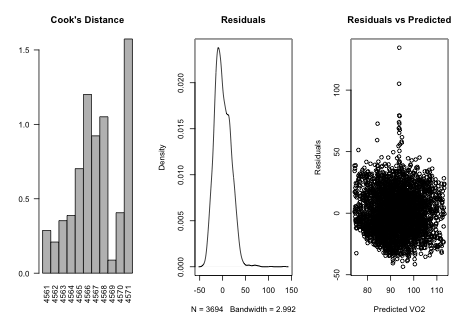
\includegraphics{figures/vo2-diagnostic-plots-1.png}
\caption{Diagnostic model plots for effects of drug treatment on VO2.
This analysis only includes HFD fed animals.}
\end{figure}

We first checked whether normality was maintained in the residuals from
the ANCOVA. These results are summarized below:

\begin{figure}[htbp]
\centering
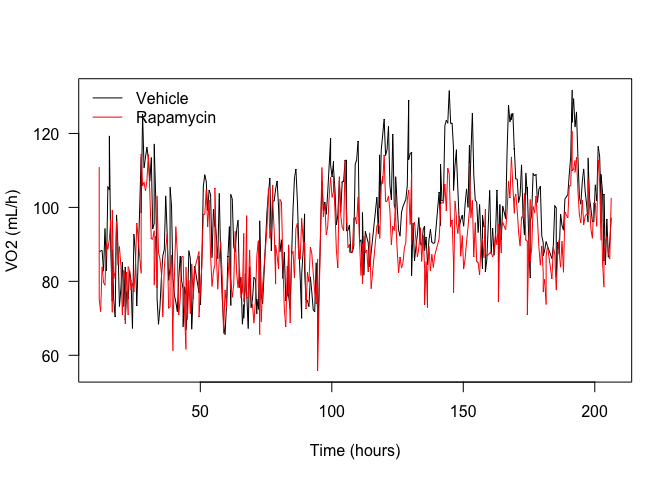
\includegraphics{figures/vo2-time-course-1.png}
\caption{Oxygen consumption over time.}
\end{figure}

This data was averaged for the VO2 before the HFD switch and after the
HFD switch

\begin{figure}[htbp]
\centering
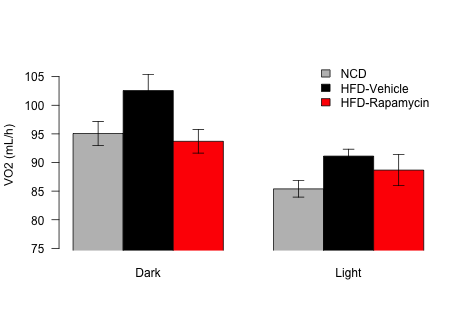
\includegraphics{figures/vo2-barplot-1.png}
\caption{Energy Expenditure Before and After High Fat Diet Treatment}
\end{figure}

Alternatively we used a mixed linear model, with non-interacting
covariates for the Light cycle, the lean mass and the treatment A
Chi-squared test comparing a model with or without the Treatment term
yielded a p-value of 6.5e-05 for the mice. This analysis excluded the
chow fed animals, and only compares HFD vehicle to HFD drug.

Based on our model, we predict the average VO2 after 14 days would be an
increase of -16.832 or -13.413\%. The model coefficients are:

\begin{longtable}[c]{@{}lrr@{}}
\caption{Model Coefficients for VO2 Mixed Linear Model}\tabularnewline
\toprule
& Coefficent & SE\tabularnewline
\midrule
\endfirsthead
\toprule
& Coefficent & SE\tabularnewline
\midrule
\endhead
(Intercept) & 134.070 & 8.664\tabularnewline
Light.DarkLight & -8.650 & 0.569\tabularnewline
Lean & -1.839 & 0.342\tabularnewline
Exp.Time & 0.107 & 0.007\tabularnewline
TreatmentRapamycin & -3.334 & 1.742\tabularnewline
Exp.Time:TreatmentRapamycin & -0.040 & 0.010\tabularnewline
\bottomrule
\end{longtable}

\subsection{Respiratory Exchange Rate}\label{respiratory-exchange-rate}

The respiratory exchange ratio is an indicator of substrate preference.
A high RER indicates preferential utilization of carbohydrates for
energy, while a low RER indicates preferential use of lipids. The normal
range of these values are 0.7 (nearly exclusivley lipid) to 1.0 (nearly
exclusively carbohydrate). Lipid utilization (low RER) is increased
during sleep (day cycle for mice).

\begin{figure}[htbp]
\centering
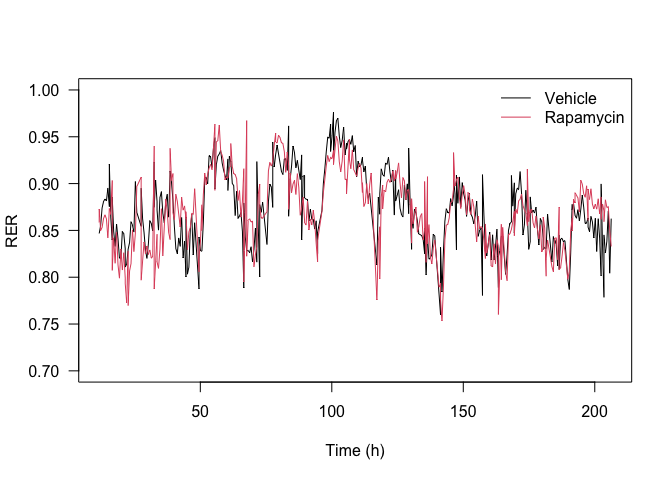
\includegraphics{figures/rer-time-course-1.png}
\caption{The respiratory exchange ratio over time.}
\end{figure}

\begin{figure}[htbp]
\centering
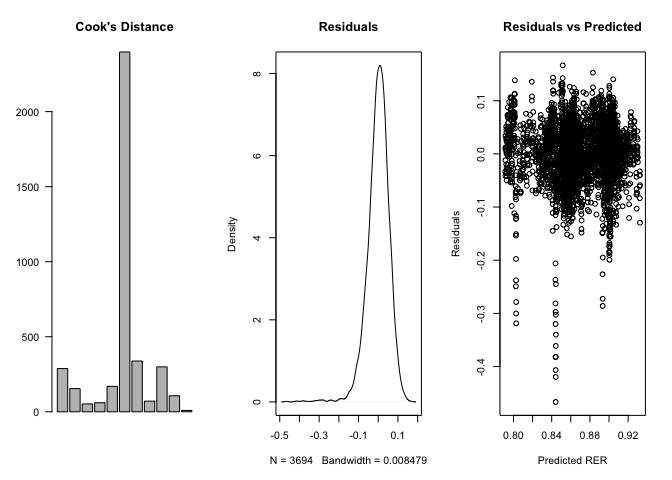
\includegraphics{figures/rer-statistics-untreated-1.png}
\caption{Diagnostic model plots for mixed linear model analysis of RER.}
\end{figure}

We used a mixed linear model, with non-interacting covariates for the
Light cycle and the treatment. A Chi-squared test comparing a model with
or without the treatment term yielded a p-value of 1.41e-02 for the
mice. This only is comparing the differnce between HFD and HFD + Drug
mice.

\begin{longtable}[c]{@{}lrr@{}}
\caption{Model Coefficients for RER Mixed Linear Model}\tabularnewline
\toprule
& Coefficent & SE\tabularnewline
\midrule
\endfirsthead
\toprule
& Coefficent & SE\tabularnewline
\midrule
\endhead
(Intercept) & 0.907155 & 0.010300\tabularnewline
Light.DarkLight & -0.042227 & 0.001862\tabularnewline
Exp.Time & -0.000140 & 0.000024\tabularnewline
TreatmentRapamycin & -0.010411 & 0.013888\tabularnewline
Exp.Time:TreatmentRapamycin & 0.000081 & 0.000033\tabularnewline
\bottomrule
\end{longtable}

\subsection{Activity Data}\label{activity-data}

Physical activity is determined via the number of beam brakes in the X
or Y direction (not vertically). These numbers are high when the mice
are awake (dark cycle) and low during the light cycle. The beam breaks
are converted into ambulatory counts based on consecutive breaks of
beams, indicating movement. These counts data are not normally
distributed and as such are typically analysed with generalized linear
models.

\begin{figure}[htbp]
\centering
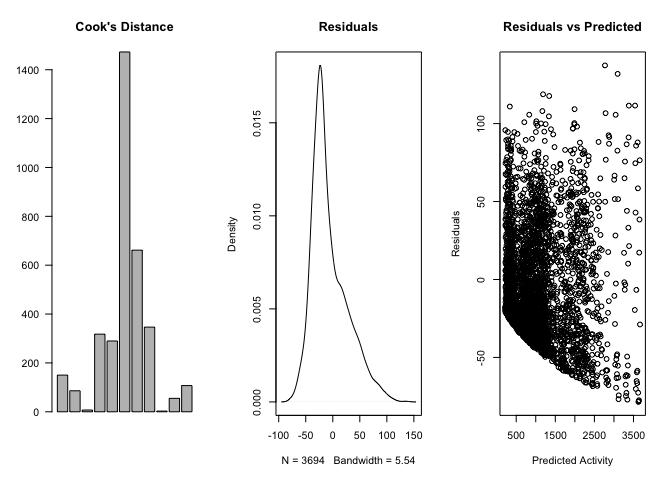
\includegraphics{figures/activity-statistics-1.png}
\caption{Model diagnostic plots for generalized linear models of
physical activity.}
\end{figure}

We used a generalized mixed linear model, with non-interacting
covariates for the Light cycle and the treatment A Chi-squared test
comparing a model with or without the Genotype term yielded a p-value of
1e+00 for the mice. This analysis used a generalized mixed linear model
(Poission) and only compares HFD to HFD + Drug.

\begin{figure}[htbp]
\centering
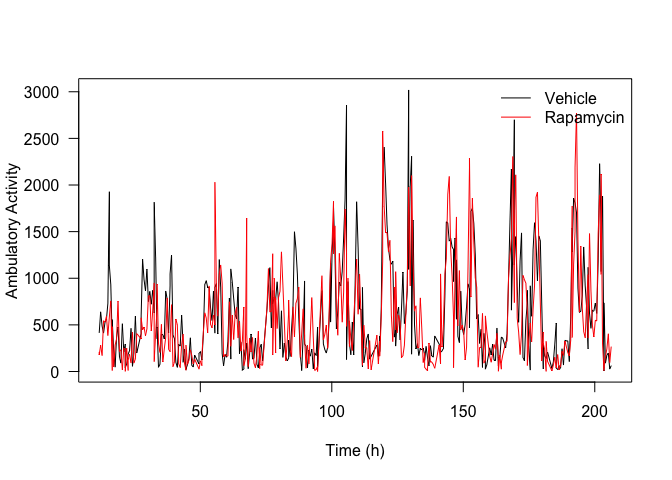
\includegraphics{figures/activity-time-course-1.png}
\caption{The activity over time.}
\end{figure}

\begin{figure}[htbp]
\centering
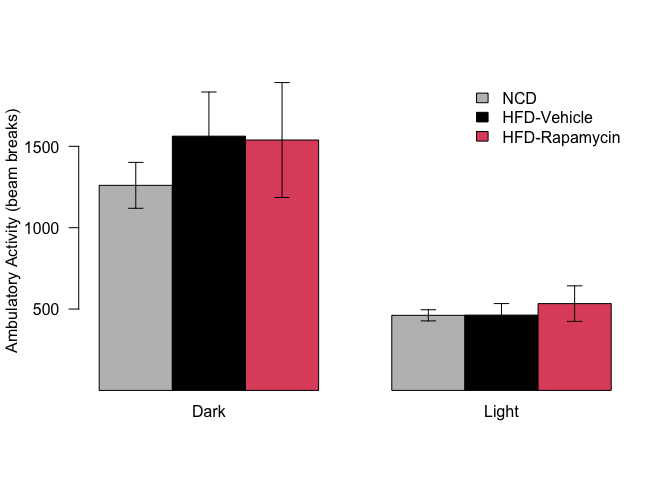
\includegraphics{figures/activity-barplot-1.png}
\caption{Physical Activity Before and After High Fat Diet Treatment}
\end{figure}

\section{Session Information}\label{session-information}

\begin{verbatim}
## R version 3.2.2 (2015-08-14)
## Platform: x86_64-apple-darwin13.4.0 (64-bit)
## Running under: OS X 10.10.5 (Yosemite)
## 
## locale:
## [1] en_US.UTF-8/en_US.UTF-8/en_US.UTF-8/C/en_US.UTF-8/en_US.UTF-8
## 
## attached base packages:
## [1] stats     graphics  grDevices utils     datasets  methods   base     
## 
## other attached packages:
##  [1] car_2.1-0          arm_1.8-6          MASS_7.3-44       
##  [4] influence.ME_0.9-6 lme4_1.1-9         Matrix_1.2-2      
##  [7] lubridate_1.3.3    dplyr_0.4.3        xlsx_0.5.7        
## [10] xlsxjars_0.6.1     rJava_0.9-7        tidyr_0.3.1       
## [13] knitr_1.11        
## 
## loaded via a namespace (and not attached):
##  [1] Rcpp_0.12.1        formatR_1.2.1      nloptr_1.0.4      
##  [4] plyr_1.8.3         highr_0.5.1        tools_3.2.2       
##  [7] digest_0.6.8       evaluate_0.8       memoise_0.2.1     
## [10] nlme_3.1-122       lattice_0.20-33    mgcv_1.8-7        
## [13] DBI_0.3.1          yaml_2.1.13        parallel_3.2.2    
## [16] SparseM_1.7        coda_0.17-1        stringr_1.0.0     
## [19] MatrixModels_0.4-1 grid_3.2.2         nnet_7.3-11       
## [22] R6_2.1.1           rmarkdown_0.8      minqa_1.2.4       
## [25] magrittr_1.5       htmltools_0.2.6    splines_3.2.2     
## [28] pbkrtest_0.4-2     assertthat_0.1     abind_1.4-3       
## [31] quantreg_5.19      stringi_0.5-5      lazyeval_0.1.10
\end{verbatim}

\end{document}
